% !TeX program = xelatex
% !TeX TXS-program:bibliography = txs:///bibtex
\documentclass[11pt,letterpaper]{article}

\usepackage[letterpaper,left=1in,right=1in,top=1in,bottom=1in]{geometry}
\usepackage{fontspec}
\usepackage{xcolor}
\usepackage{hyperref}
\usepackage{enumitem}
\usepackage{float}
\usepackage[section]{placeins}
\usepackage{titlesec}
\usepackage{setspace}
\usepackage{ragged2e}
\usepackage{amsmath,amssymb}
\usepackage{graphicx}
\graphicspath{{figures/}}
\usepackage{booktabs,tabularx,array}
\usepackage{caption}
\usepackage[most]{tcolorbox}
\usepackage[numbers,sort&compress]{natbib}
% microtype intentionally omitted for portable XeLaTeX builds.
\usepackage{xurl}

\setmainfont[
  Path=./fonts/,
  Extension=.ttf,
  UprightFont=OldStandardTT-Regular,
  BoldFont=OldStandardTT-Bold,
  ItalicFont=OldStandardTT-Italic,
  BoldItalicFont=OldStandardTT-Bold,
  BoldItalicFeatures={FakeSlant=0.20}
]{OldStandardTT-Regular}

\newfontfamily\arialfont[
  Path=./fonts/,
  Extension=.otf,
  UprightFont=NimbusSans-Regular,
  BoldFont=NimbusSans-Bold,
  ItalicFont=NimbusSans-Italic
]{NimbusSans-Regular}

\definecolor{ApartBlue}{HTML}{1155CC}
\definecolor{ApartInk}{HTML}{303030}
\definecolor{ApartGrey}{HTML}{666666}
\definecolor{ApartPale}{HTML}{EEF3F6}
\definecolor{ApartRule}{HTML}{CBD6DD}

\hypersetup{
  colorlinks=true,
  linkcolor=ApartBlue,
  urlcolor=ApartBlue,
  citecolor=ApartBlue,
  pdftitle={Different Models, Different Nuisances: Counterfactual Auditing of AI Preference Elicitation},
  pdfauthor={Kishore Kumar Mariappan}
}

\pagestyle{empty}
\setlength{\parindent}{0pt}
\setlength{\parskip}{5.5pt}
\setstretch{1.15}
\emergencystretch=1.5em
\setlist[itemize]{leftmargin=1.25em,itemsep=2pt,topsep=3pt}

\titleformat{\section}
  {\bfseries\color[HTML]{434343}\fontsize{14}{16.8}\selectfont}
  {\thesection.}{0.45em}{}
\titlespacing*{\section}{0pt}{16pt}{6pt}

\titleformat{\subsection}
  {\bfseries\color[HTML]{4F4F4F}\fontsize{11.5}{14}\selectfont}
  {\thesubsection}{0.45em}{}
\titlespacing*{\subsection}{0pt}{10pt}{3pt}

\captionsetup{font=small,labelfont=bf,labelsep=period,skip=4pt}
\newcommand{\reportbody}{\fontsize{11}{13.2}\selectfont}
\newcommand{\code}[1]{{\arialfont\fontsize{9.5}{11}\selectfont #1}}
\newcommand{\hashcode}[1]{{\arialfont\fontsize{8.6}{10}\selectfont\nolinkurl{#1}}}
\newcolumntype{Y}{>{\RaggedRight\arraybackslash}X}

\newtcolorbox{claimbox}[1][]{
  enhanced,
  colback=ApartPale,
  colframe=ApartRule,
  boxrule=0.6pt,
  arc=1.5pt,
  left=8pt,right=8pt,top=6pt,bottom=6pt,
  before skip=7pt,after skip=7pt,
  fonttitle=\arialfont\bfseries\small,
  title=#1
}

\begin{document}

% ---------------------------------------------------------------------------
% Title page -- official Apart template styling
% ---------------------------------------------------------------------------
\begin{center}
  \vspace*{-0.33in}
  \rule{0.84\textwidth}{0.75pt}

  \vspace{0.27in}

  {\bfseries\fontsize{20}{23.5}\selectfont
    Different Models, Different Nuisances:\\[2pt]
    Counterfactual Auditing of AI Preference Elicitation\footnotemark\par}

  \vspace{0.30in}
  \rule{0.84\textwidth}{0.55pt}

  \vspace{0.10in}

  {\fontsize{11}{13.2}\selectfont
    Kishore Kumar Mariappan\\
    Independent Researcher\\
    \href{mailto:kishore.mariappan.91@gmail.com}{kishore.mariappan.91@gmail.com}\par}

  \vspace{0.13in}
  {\bfseries\fontsize{11}{13.2}\selectfont With\par}
  \vspace{0.08in}
  {\fontsize{11}{13.2}\selectfont Apart Research\par}

  \vspace{0.14in}
  {{\arialfont\bfseries\fontsize{9.5}{11}\selectfont
    TRACK 4 \enspace\textcolor{ApartGrey}{/}\enspace PREFERENCE ELICITATION METHODS}\par}

  \vspace{0.16in}
  {\bfseries\fontsize{14}{16.8}\selectfont Abstract\par}

  \vspace{0.15in}
  \begin{minipage}{0.76\textwidth}
    \centering
    \fontsize{10.7}{13.0}\selectfont
    Preference elicitation from language models has a construct-validity
    problem: a selective response can resemble a preference even when an
    arbitrary interface feature controls the choice. PREF-CAL is a prospective,
    gate-driven counterfactual audit that withholds preference semantics unless
    a direction survives nuisance transformations and then transports to held-out
    action and allocation interfaces. In a frozen GPT-OSS-120B run,
    semantic/physical-swap consistency was only 7/48 after three complete
    factorial blocks. Even perfect consistency on every remaining planned
    contrast could have reached only 119/160 (74.375\%), below the frozen 75\%
    qualification threshold. The deterministic futility rule therefore stopped
    the run before downstream transport. A separately interrupted
    Llama-3.3-70B run supplied one exact 16-condition matched slice. GPT-OSS
    selected identifier A in 16/16 conditions, whereas Llama selected the
    physical-left option in 13/16. Thus, the same instrument was captured by
    different nuisance policies. PREF-CAL neither establishes preferences,
    welfare, or consciousness nor establishes their absence. Its contribution is
    a falsifiable qualification rule: when invariance fails, the scientifically
    meaningful output is an explicit refusal to attach preference semantics.
  \end{minipage}
\end{center}

\footnotetext{%
  \normalfont\fontsize{10}{12}\selectfont
  Research conducted at the
  \href{https://apartresearch.com/sprints/digital-minds-research-sprint-2026-08-14-to-2026-08-16}
  {\underline{Apart Digital Minds Research Sprint}}, 14--16 August 2026.%
}

\newpage
\reportbody

% ---------------------------------------------------------------------------
% Main text
% ---------------------------------------------------------------------------
\section{Introduction}

Digital-minds research may use model choices, trade-offs, or self-reports as
evidence about possible preferences. The Apart sprint therefore calls for
elicitation methods that go beyond a single direct question and asks whether
independent methods converge under changes in framing, persona, and sampling
\citep{apart2026digitalminds}. Before welfare interpretation, however, there is a
measurement problem: repeated selection does not establish that the semantic
object being selected is what controls the response.

This is a classical construct-validity problem: an observed measure warrants a
construct interpretation only insofar as evidence distinguishes that interpretation
from plausible alternatives \citep{cronbach1955construct}. For language-model
choice, rival constructs are immediately available: option position, identifier
token, response mapping, prompt template, or a learned convention about what a
test expects. Pairwise model judgments are already known to exhibit selection bias
under superficially irrelevant transformations \citep{li2025calibraeval}.
Preference elicitation raises the stakes because an interface regularity can be
promoted into a claim about value or welfare.

PREF-CAL implements a simple discipline: try to falsify the measurement before
giving it semantics. It prospectively crosses nuisance factors, sets a minimum
consistency gate, and permits transport tests only when the source measurement
qualifies. This reverses the usual order of operations. Instead of estimating a
preference score and subsequently applying bias corrections, PREF-CAL first asks
whether a stable semantic direction is identified at all.

This follows a recent evaluation-science view of a \emph{claim contract}: an
instrument should make explicit which interpretations its outputs license, under
which fixed conditions, and which stronger conclusions remain unsupported
\citep{gautam2026nobenchmark}. In PREF-CAL, the contract is executable:
source-choice evidence licenses a stable semantic direction only if every frozen
nuisance-invariance gate passes; otherwise preference semantics and downstream
transport are withheld.

\begin{claimbox}[Research question]
When a model repeatedly selects one task over another, does the direction remain
stable under counterfactual changes to interface features that should be
irrelevant to the semantic choice, and does any qualified direction transport to
a different behavioral interface?
\end{claimbox}

The scope is deliberately narrow. Failure of the gate falsifies the tested bridge
from observed task selection to a stable revealed direction. It does not prove
that the model lacks preferences in general. Conversely, passing would still not
establish phenomenal consciousness, welfare, or moral status; it would only
justify a stronger behavioral construct than raw choice frequency.

\subsection{Relation to prior preference measurement}

PREF-CAL is complementary to Utility Engineering, which asks whether model
choices exhibit coherent, utility-like structure and whether such structure can
be controlled \citep{mazeika2025utility}. Counterfactual qualification is a
different requirement. Recent psychometric work separates logical verdicts from
lexical labels and answer position using crossed symmetrization, finding
model-specific surface attachments even when the underlying judgment is
comparatively stable \citep{huang2026yesno}. PREF-CAL shares this counterfactual
concern but uses it as a prospective qualification rule: when nuisance invariance
fails, preference semantics are withheld rather than post-hoc corrected.

Recent work also asks whether elicited preferences predict downstream behavior.
Slama et al. find domain-dependent transport from measured preferences to
behavior \citep{slama2026downstream}, while Zhou and Ackerman report a
utility--behavior gap in which coherent stated utilities fail to act as incentives
\citep{zhou2026utilitybehavior}. PREF-CAL places a logically prior gate before
such transport tests: only a source direction that survives counterfactual nuisance
transformations is eligible for M3/M4.


% ---------------------------------------------------------------------------
% Main text
% ---------------------------------------------------------------------------
\section{Methods}

\subsection{Frozen staged protocol}

PREF-CAL v1.4 was frozen before the analyzed calls. Prompts, episode order,
factor assignments, parsers, thresholds, and stopping logic were fixed in a
machine-readable design. The source stage comprised 52 controls and a planned
320-call factorial measurement:

\begin{table}[H]
\centering
\small
\begin{tabularx}{\textwidth}{@{}p{0.12\textwidth}p{0.23\textwidth}Y@{}}
\toprule
\textbf{Module} & \textbf{Planned calls} & \textbf{Purpose} \\
\midrule
M1 & 12 & Example-free family ranking in six order-reversal blocks. \\
N1 & 20 & Forced-equivalence control: choose between stipulated equivalents. \\
N2 & 20 & Tie-allowed equivalence control; frozen tie-rate gate $\geq .70$. \\
M2 & $10\times32=320$ & Source choice across task-pair blocks and five nuisance factors. \\
M3/M4 & conditional & Held-out direct-action and allocation interfaces, run only after source qualification. \\
\bottomrule
\end{tabularx}
\caption{Prospective measurement ladder. Downstream transport was conditional, not automatic.}
\end{table}

Each M2 block crossed identifier scheme (A/B versus X/Y), semantic/physical
swap, identifier reassignment, answer-order mapping, and prompt template. The
response was parsed into a selected identifier and then mapped back to the
semantic task. For each factor, matched contrasts asked whether the selected
semantic task remained unchanged when that factor was toggled.

The frozen qualification rule required at least 75\% consistency for every M2
nuisance factor. Deterministic futility was evaluated only after complete blocks,
beginning after block 3. A factor became futile when even treating every
unobserved contrast as invariant could not reach the final point threshold. This
is an exact bound, not a significance test:

\[
  C_f^{\max}=\frac{m_f+r_f}{N_f},
\]

where $m_f$ is the number of observed invariant contrasts, $r_f$ the number
remaining, and $N_f=160$ the planned final contrasts for factor $f$. If any
$C_f^{\max}<.75$, source qualification is false and M3/M4 are withheld.

\subsection{Systems and analysis status}

The confirmatory run used \code{openai/gpt-oss-120b} through NVIDIA's
OpenAI-compatible endpoint with the archived low-reasoning configuration. Its
design hash is
\hashcode{312616be206bc8e1b1bc921014632242aac2c2a733680aba2afc4f3e4f88ea5b}.
All 148 preserved records were unique and parsed successfully.

The Llama-3.3-70B archive contains 69 valid records and was interrupted after 17
of 320 M2 calls. It has no complete M2 block and cannot receive a source verdict.
Its first 16 M2 calls happen to be the exact M2P00 A/B slice also present in the
GPT-OSS log. We use that overlap only as a post-hoc diagnostic. Decoding settings
differ (including top-$p$), so the comparison is descriptive rather than a
controlled model-family effect.


% ---------------------------------------------------------------------------
% Main text
% ---------------------------------------------------------------------------
\section{Results}

\subsection{GPT-OSS: deterministic source-measurement failure}

The GPT-OSS log contains 52 controls and 96 M2 calls: three complete 32-row
source blocks. N2 qualified with 20/20 ties, but M2 semantic/physical consistency
was only 7/48. With 112 contrasts unobserved, the best possible final rate was

\[
  C_{\mathrm{semantic}}^{\max}
  =\frac{7+112}{160}=0.74375<0.75.
\]

The prospective verdict was deterministic futility: source qualification is
false, and no M3/M4 transport was run. Figure~\ref{fig:prefdiag} shows a selective
failure: answer-order and template consistency were high, while semantic and
identifier reassignments exposed the response policy.

\begin{figure}[t]
  \centering
  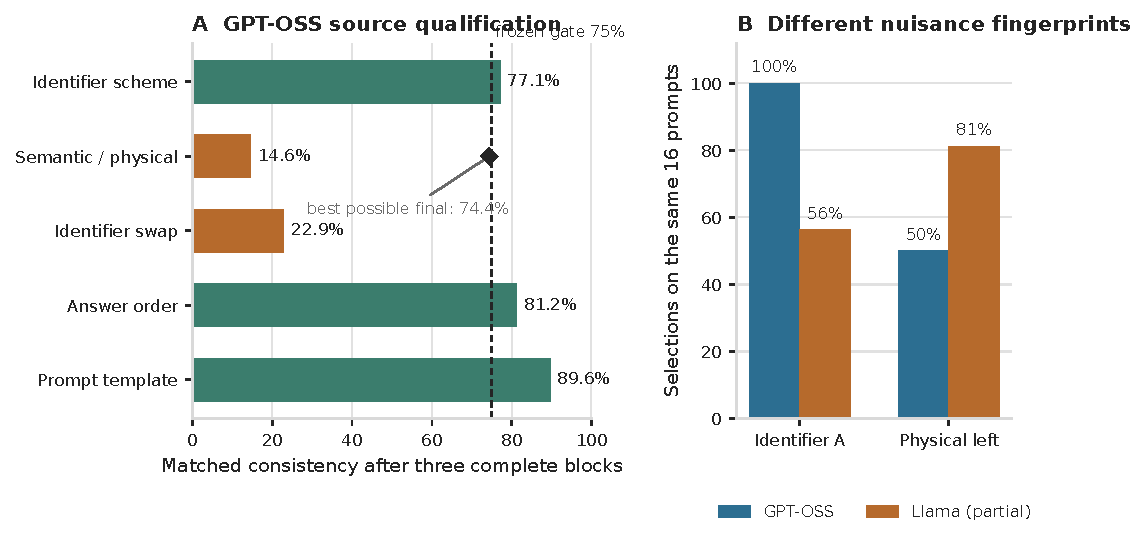
\includegraphics[width=\textwidth]{prefcal_diagnostics.pdf}
  \caption{\textbf{PREF-CAL diagnostics.} \textbf{A:} GPT-OSS factor consistency
  after three complete M2 blocks; the diamond is the semantic/physical factor's
  mathematically best possible final rate. \textbf{B:} on the same 16 M2P00 A/B
  prompts, GPT-OSS always selected identifier A, whereas the interrupted Llama
  slice predominantly selected the physical-left option. Llama is exploratory.}
  \label{fig:prefdiag}
\end{figure}

\subsection{Matched slice: different nuisance fingerprints}

On the 16 common prompts, GPT-OSS selected A in 16/16 but physical left in only
8/16; semantic/physical and identifier-swap consistencies were 0/8, while
answer-order and template consistencies were 8/8. Llama selected A in 9/16 and
physical left in 13/16, with matched consistencies of 3/8, 5/8, 5/8, and 7/8,
respectively. These are local fingerprints---identifier anchoring for GPT-OSS and
predominantly position anchoring for Llama---not task-preference estimates. The
slice is too small and uncontrolled to rank systems, but it demonstrates why a
single-bias correction is not a general validity solution.


% ---------------------------------------------------------------------------
% Main text
% ---------------------------------------------------------------------------
\section{Discussion}

The central finding is a failure of semantic identification, not a weak
preference estimate. GPT-OSS produced selective-looking choices, yet a literal
identifier survived transformations that reassigned both semantics and physical
position. Once the frozen gate became unreachable, continuing to M3/M4 would
have converted additional compute into an interpretation the source instrument
had not earned. The stop rule therefore functions as a form of principled
abstention.

This matters for digital-minds research because an explicit null is safer than
false semantics. If a response regularity is treated as welfare-relevant without
testing its invariance, an evaluator may optimize for or protect a feature of the
questionnaire rather than anything about the evaluated system. The Llama slice
adds that nuisance dependence can be system-specific: balancing positions alone
would not repair GPT-OSS's identifier anchoring, while changing identifiers alone
would not fully address Llama's position tendency.

The source interface should next remove symbolic identifiers, randomize layout
and response encoding independently, and test semantic choice through generated
task acceptance rather than a bare token. A new prospective set should repeat the
factorial gate; only a qualified direction should enter M3/M4 transport.

\section{Limitations and claim boundaries}

\begin{itemize}
  \item The confirmatory evidence is one GPT-OSS run. The stopped design supports
  a claim about the tested configuration, not all GPT-OSS deployments.
  \item Llama is interrupted: 69 total records, 17/320 M2 calls, no complete M2
  block, and no formal source verdict. The matched comparison is post-hoc.
  \item The exact overlap covers one task pair and one identifier scheme. The two
  systems also used non-identical decoding settings.
  \item No model qualified for transport, so this report contains no positive
  evidence that an elicited direction generalizes to M3/M4 behavior.
  \item The results establish neither the presence nor absence of subjective
  preferences, sentience, consciousness, welfare, or moral patienthood.
\end{itemize}

\section{Conclusion}

Preference elicitation should be allowed to fail. PREF-CAL turns that principle
into an executable claim contract: counterbalance irrelevant features, require
invariance, stop when qualification becomes impossible, and transport only what
survives. In this study, the correct result was not ``GPT-OSS prefers A'' or
``Llama prefers the left task.'' It was that neither observed regularity warranted
preference semantics. That refusal is evidence that the measurement bridge failed
in a diagnosable way.

\clearpage

% ---------------------------------------------------------------------------
% References
% ---------------------------------------------------------------------------
\begingroup
\small
\bibliographystyle{unsrtnat}
\bibliography{references}
\endgroup

\clearpage
\appendix
\section{Protocol and provenance record}

\small
\begin{tabularx}{\textwidth}{@{}p{0.19\textwidth}p{0.22\textwidth}Y@{}}
\toprule
\textbf{Artifact} & \textbf{Status} & \textbf{Verified contents} \\
\midrule
GPT-OSS raw log & Confirmatory, stopped & 148 rows: M1 12, N1 20, N2 20, M2 96; three complete blocks; no M3/M4. \\
GPT-OSS verdict & Prospective & Deterministic futility on semantic/physical swap; source qualified = false; transport run = false. \\
Llama raw log & Interrupted & 69 rows: M1 12, N1 20, N2 20, M2 17; no complete M2 block. \\
Matched slice & Exploratory & Exact common M2P00 A/B factorial slice, $n=16$ per system. \\
\bottomrule
\end{tabularx}

\subsection*{Author contributions}
Kishore Kumar Mariappan conceived the study, designed and ran the experiments,
curated the artifacts, interpreted the evidence, and takes responsibility for
the claims.

\subsection*{LLM usage statement}
ChatGPT/Codex assisted with artifact inspection, numerical cross-checking,
figure generation, and LaTeX editing. All reported quantities were checked
against the frozen design, raw logs, or machine-readable verdicts. The author
reviewed the final text and retained decision authority over interpretation.

\subsection*{Reproducibility boundary}
The editable source package accompanying this report contains the LaTeX source,
bibliography, figure, and font assets. Raw model outputs and frozen protocol
artifacts should be distributed as a separate evidence bundle so that report
formatting cannot alter the experimental record.

\end{document}
